\documentclass[letter,11pt]{article}
\usepackage[spanish, mexico, activeacute]{babel}
\usepackage{amsfonts}
\usepackage{amsmath,amsfonts,amssymb}
\usepackage{fancyhdr}
\usepackage{fancyvrb}
\usepackage{xy}
\usepackage{graphicx}
\usepackage{latexsym,amsfonts}
\usepackage{enumerate}
\usepackage[spanish,activeacute]{babel}
\usepackage{multirow}
\usepackage{multicol}
\usepackage{hyperref}

\textwidth 160mm
\textheight 235mm
\oddsidemargin 0.7cm
\topmargin -1cm


\usepackage[numbered,framed]{matlab-prettifier}
\lstMakeShortInline"
\lstset{
  style              = Matlab-editor,
  %basicstyle         = \mlttfamily,
  escapechar         = ",
  mlshowsectionrules = true,
}


\setlength{\oddsidemargin}{-0.5cm}
\setlength{\evensidemargin}{0cm} \setlength{\textwidth}{17.5cm}
\setlength{\textheight}{24cm} \setlength{\topmargin}{-1.7cm}
\newcommand{\N}{\mathbb{N}}

\title{lab01 521230 2018-1}

\addtolength{\voffset}{-1cm}

%\pagestyle{empty}

\parindent 0cm

\font\bff=cmbx10 at 10truept
\font\lg=cmdunh10 at 10truept
\font\bl=cmss10 at 10truept

\newcommand\R{\mathbb{R}}
\newcommand\IN{\mathbb{N}}
\newcommand\Z{\mathbb{Z}}
\newcommand\bsi{{\mbox{\boldmath $\sigma$}}}
\newcommand\bta{{\mbox{\boldmath $\tau$}}}
\newcommand\bet{{\mbox{\boldmath $\eta$}}}
\newcommand\bga{{\mbox{\boldmath $\gamma$}}}
\newcommand\bze{{\mbox{\boldmath $\zeta$}}}
\newcommand{\dis}{\displaystyle}

\renewcommand\u{\mathbf{u}}
\newcommand\bv{\mathbf{v}}
\newcommand\0{\mathbf{0}}

\newcommand\I{\mathbf{I}}
\def\e{\mathbf{e}}
\def\qen{{\quad\hbox{en}\quad}}
\newcommand\f{\mathbf{f}}
\newcommand\disp{\displaystyle}
\newcommand\bdiv{\mathbf{div}\,}
\newcommand\bnu{{\mbox{\boldmath $\nu$}}}
\renewcommand\div{\mathrm{div}\,}
\newcommand\tr{\mathrm{tr}\,}
\newcommand{\matlab}{{\sc Matlab }}

\newcommand{\header}{
{\lg UNIVERSIDAD DE CONCEPCION}\hfill
\vskip-4truept
{\bff FACULTAD DE CIENCIAS}\hfill
\vskip-4truept
{\bff FISICAS Y MATEMATICAS}\hfill
\vskip-4truept
{\bl DEPARTAMENTO DE INGENIERIA MATEMATICA}\hfill
\vskip4truept\hrule\hrule\vskip4truept
\par
}

\begin{document}
\header
\vspace{0.7cm}
\begin{center}
\textbf{\small C\'alculo Num\'erico (521230) - Laboratorio 1}\\
\vspace{0.1cm}
\textbf{\Large INTRODUCCION A MATLAB I}
\vspace{0.7cm}
\end{center}

\matlab{} es una abreviatura para matrix laboratory (laboratorio de matrices).
\'Este es un programa (y a la vez un lenguaje de programaci\'on)
especialmente dise\~nado para la soluci\'on num\'erica de problemas
matem\'aticos como, por ejemplo, sistemas de ecuaciones lineales, sistemas
de ecuaciones no lineales, problemas de valores iniciales, etc.

La p\'agina web del programa es \verb"http://es.mathworks.com/index.html". En ella
se encuentran ejemplos de aplicaci\'on del programa para la soluci\'on de distintos
tipos de pro\-ble\-mas reales, videos y documentaci\'on.

\section{Generalidades}



%\begin{enumerate}

\textbf{Observaci\'on:} Si bien las gu\'ias de estos laboratorios hacen referencia a la versi\'on de \matlab{} R2013a, para el S.O. \emph{Linux} instalado en los laboratorios LC 301 y LC 304 de la Facultad de Ciencias F\'isicas y Matem\'aticas, lo que se ver\'a aqu\'i, puede ser aplicable a versiones m\'as recientes de \matlab, versiones un poco mas antiguas o versiones en otras plataformas como \emph{Windows} o \emph{Mac}.

\medskip

Para comenzar \matlab, en la esquina superior izquierda: 		\verb+Inicio > Desarrollo > Matlab R2013a+, como lo muestra la figura \ref{fig:inicio_matlab}.

\begin{figure}[h]
\centering
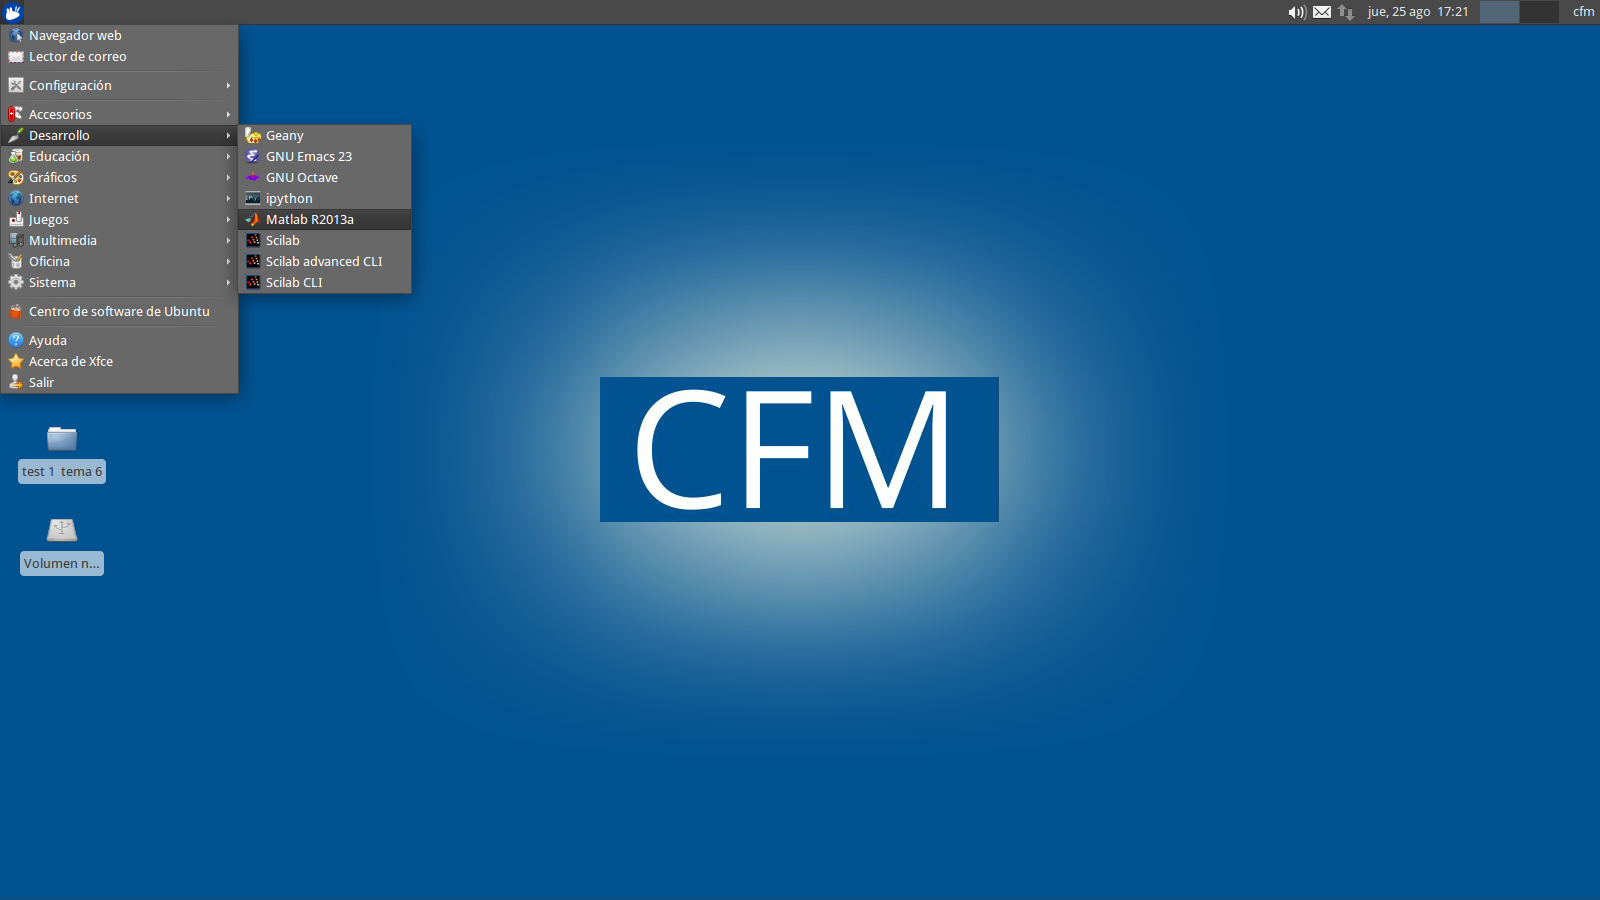
\includegraphics[width=0.8\textwidth]{menu.png}
\caption{Men\'u para iniciar \matlab.}\label{fig:inicio_matlab}
\end{figure}

\newpage

Aparecer\'a el logo de \matlab{} mientras inicia el programa, como se muestra en la figura \ref{fig:logo_matlab}. 

\begin{figure}[h]
\centering

\includegraphics[width=0.8\textwidth]{inicio_matlab.png}
\caption{Logo de \matlab.}\label{fig:logo_matlab}
\end{figure}

Una vez iniciado \matlab{} lo que ver\'a ser\'a la interfaz gr\'afica (layout) por defecto mostrada en la figura \ref{fig:layout_matlab}. En caso de que no aparezca una interfaz como la de la figura \ref{fig:layout_matlab}, haga click en el bot\'on \emph{Layout} (aparece en el men\'u de la barra superior, aproximadamente en la mitad) y posteriormente en la opci\'on \emph{Default}.

\begin{figure}[h]
\centering
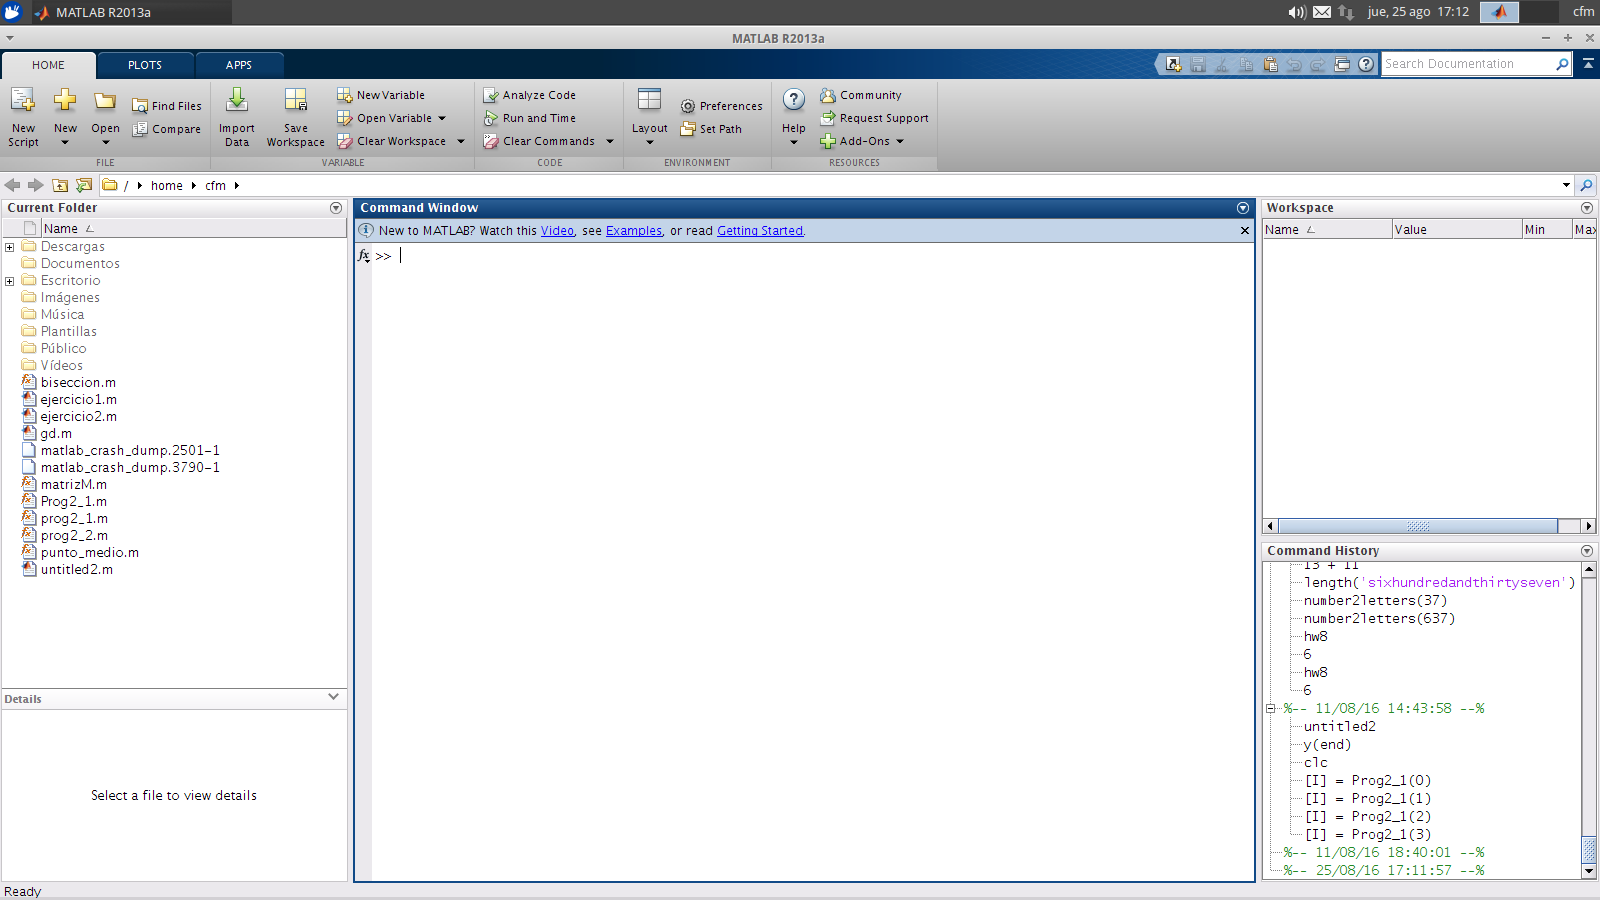
\includegraphics[width=0.8\textwidth]{layout_matlab.png}
\caption{Interfaz gr\'afica (layout) de \matlab.}\label{fig:layout_matlab}
\end{figure}

Puede notar que aparecen 5 ventanas en esta interfaz:

\begin{enumerate}
\item \emph{Current Folder}: Esta ventana muestra el contenido de la carpeta donde trabaja \matlab. La direcci\'on de esta carpeta se puede apreciar inmediatamente arriba, en la barra de navegaci\'on. La carpeta por defecto en la cual trabaja matlab es \verb"/home/cfm", aunque esta puede ser cambiada en la misma barra de navegaci\'on o haciendo click en alguna de las carpetas que muestra esta ventana.
\item \emph{Details}: Esta ventana muestra propiedades de los archivos que se seleccionan en \emph{Current Folder}, similar a las ventanas de Windows.
\item \emph{Command Window} (Ventana de Comandos):  La ventana principal de \matlab. En esta ventana se ejecutan todos los comandos, operaciones, asignaciones y programas de \matlab. Para ejecutar una instrucci\'on, se escribe esta instucci\'on y se presiona la tecla \emph{Enter}. Si en la ventana de comandos de \matlab{} escribimos una instrucci\'on seguido por \verb+;+, \matlab{}	no mostrar\'a el resultado de la operaci\'on realizada.		
\item \emph{Workspace}: Esta ventana muesta las variables que actualmente estan guardadas en la memoria temporal de \matlab. En cualquier momento del trabajo con \matlab, escribiendo el comando \Verb+whos+ en la ventana de comandos podremos ver	las variables en memoria y con el comando \Verb+clear all+ o \verb"clear <nombre_variable>" podremos eliminarlas de memoria, aunque tambi\'en se puede eliminar haciendo click con el boton derecho del mouse en la variable y seleccionando la opci\'on \emph{Delete}.
\item \emph{Command History}: Muestra el historial de los \'ultimos comandos ejecutados (correcta o incorrectamente) en la ventana de comandos. Se puede volver a ingresar un comando haciendo doble click sobre este, o bien en la ventana de comandos apretando reiteradas veces la flecha hacia arriba del teclado  hasta encontrar el comando, y luego presionar la tecla \emph{Enter}.
\end{enumerate}

Para salir de \matlab{} se puede ingresar \verb+exit+ o \verb+quit+ en la ventana de comandos, o bien haciendo click en la $\times$ que aparece en la esquina superior derecha.

Se puede acceder a la ayuda  en \matlab{} ingresando \verb+helpdesk+ o \verb+helpwin+ o \verb+help <nombre_comando>+ en la ventana de comandos o haciendo click en el bot\'on \emph{Help} en la barra de men\'u.
%		\index{ayuda en matlab}
	
% 	\item En cualquier momento del trabajo con \matlab, con el comando \Verb+whos+ podremos ver
% 		las variables en memoria y con el comando \Verb+clear all+ podremos eliminarlas de memoria.
% 		\index{whos}\index{clear all}
% 		
% 	\item Cuando en \matlab\, realizamos una operaci\'on y no asignamos el resultado a ninguna variable,
% 		la respuesta se asigna a una variable especial llamada \Verb+ans+.
% 		\index{ans}
		
%	\item 
%\end{enumerate}





En las secciones que contin\'uan se ver\'an los comandos necesarios para comenzar a utilizar \matlab\,
para la soluci\'on de los problemas matem\'aticos que veremos durante el semestre.
Los comandos encerrados en recuadros deben ser escritos en la ventana de comandos.
Las palabras que siguen a un signo \texttt{\%} son s\'olo comentarios
para explicar un comando particular y no tienen que ser escritas en la ventana de comandos de \matlab.

\bigskip
\centerline{\textsc{Trabajo con n\'umeros reales}}
\medskip

	En \matlab\, es posible realizar todas las operaciones aritm\'eticas entre n\'umeros reales.
	En el cuadro \ref{table:operaciones} se muestran los comandos para realizarlas.
	\index{operadores aritm\'eticos}

	\begin{table}[ht]
\begin{center}
		\begin{tabular}{|c|c|}\hline
			\verb@ + @ & adici\'on\\\hline
			\verb@ - @ & sustracci\'on\\\hline
			\verb+ * + & producto\\\hline
			\verb+ / + & divisi\'on\\\hline
			\verb+ ^ + & potencia\\\hline
		\end{tabular}
\end{center}
		\caption{Comandos para operaciones aritm\'eticas}\label{table:operaciones}
	\end{table}

	Cuando, como en el recuadro que sigue, realizamos una operaci\'on en \matlab\, y no asignamos el resultado a ninguna variable, la respuesta se asigna a una variable especial llamada \verb+ans+.

	\medskip
	
	\begin{lstlisting}
>> 10.5 + 3.1    % suma de dos números reales, el resultado se asigna a ans
	\end{lstlisting}
\newpage

	Tambi\'en podemos, con el comando \Verb+ = +
	asignar n\'umeros reales a variables.
		
	El comando \Verb+whos+ muestra las variables almacenadas en memoria.
	
	\medskip
	%de asignación
	\begin{lstlisting}
>> a = 10.5+3.1;  % no se muestra resultado de asignación
>> b = 1/5        % se muestra resultado de asignación

>> a + b
>> a*b^3          % Primero se calcula potencia cúbica de b
>> (a*b)^3        % Primero se multiplican a y b

>> whos           % sólo a, b y ans deberían estar en memoria
	\end{lstlisting}
	
	\medskip
				
	El comando \Verb+format+ permite cambiar la forma en que el valor
	de una variable se muestra en pantalla. Tenga siempre presente
	que con este comando s\'olo se cambia la forma en que se muestra el valor de
	la variable, no se cambia el valor de la variable.
	En \matlab\, los n\'umeros reales se muestran por defecto en formato \Verb+short+.
	\index{format}
    \medskip

\begin{lstlisting}
>> a              % ver el valor de a con formato por defecto
>> format long    % cambiar formato a long
>> a
>> format rat     % cambiar formato a rat
>> a
>> format short   % cambiar formato a short
>> a
\end{lstlisting}

\medskip
	
	En la tabla \ref{table:compare} se encuentran los comandos que se utilizan en
	\matlab\, para comparar dos n\'umeros reales. El resultado de la comparaci\'on
	ser\'a \Verb+1+ (si la proposici\'on es verdadera) o \Verb+0+ (si la proposici\'on es falsa).	
	
	\begin{table}[ht]
\begin{center}
		\begin{tabular}{|c|c|}\hline
			\Verb+ == + & igual a\\\hline
			\Verb+ > + & mayor que\\\hline
			\Verb+ < + & menor que\\\hline
			\Verb+ >= + & mayor o igual que\\\hline
			\Verb+ <= + & menor o igual que\\\hline
			\Verb+ ~= + & distinto de\\\hline
		\end{tabular}
\end{center} 			
		\caption{Comparaciones entre n\'umeros reales en \matlab}\label{table:compare}
	\end{table}

Los comandos \Verb+&&+, \Verb+||+ y \Verb+~+
	representan los operadores l\'ogicos conjunci\'on ($\wedge$),
	disyunci\'on ($\vee$) y negaci\'on ($\sim$) respectivamente.	
	\index{comparaciones entre n\'umeros reales}\index{operadores l\'ogicos}

	
	\begin{table}[ht]
\begin{center}
		\begin{tabular}{|c|c|}\hline
			\Verb+ && + & $\wedge$\\\hline
			\Verb+ || + & $\vee$\\\hline
			\Verb+ ~ + & $\sim$\\\hline
		\end{tabular}
\end{center}
\caption{Conectivos l\'ogicos en \matlab}\label{table:logic}
\end{table}

\newpage
\begin{lstlisting}
>> c = 3/4             % asignamos 3/4 a la variable c
>> b == c              % b igual a c
>> (a > b) && (b > c)  % (a mayor que b) y (b mayor que c)
>> ~(a <= b || a <= c) % negación de:
% (a menor o igual que b) o (a menor o igual que c)
\end{lstlisting}

\medskip

Muchas de las funciones conocidas ya est\'an incorporadas en \matlab.
Observe que la cons\-tan\-te \Verb+pi+ contiene un valor aproximado de $\pi$.
\index{abs}\index{cos}\index{sin}\index{pi}\index{log}\index{exp}\index{log2}
\index{sqrt}

\medskip

\begin{lstlisting}
>> abs(-3/5)      % valor absoluto de un número real
>> sqrt(9)        % raiz cuadrada de un numero real positivo
>> format long
>> pi
>> format rat
>> pi             % pi se trabaja con una aproximacion racional
>> format short

>> cos(pi/2)      % ¿es cero el resultado?
>> sin(pi/4)
>> d = sqrt(2)    % raíz cuadrada de un número real

>> log2(d)        % logaritmo base 2 de un número real	

>> x = 1/6
>> y = exp(x)     % función exponencial		
>> format rat
>> log(y)         % logaritmo natural de un número real
>> format short
\end{lstlisting}

\medskip

	En los computadores personales se utiliza la aritm\'etica de punto flotante para
	almacenar los n\'umeros reales. En \matlab\, cada n\'umero real se almacena en formato {\em double}, es decir,
	usando 64 bits consecutivos de memoria.
    
Las constantes \texttt{realmax} y \texttt{realmin} contienen el mayor
n\'umero real positivo y el menor n\'umero real positivo normalizado que
pueden almacenarse de esta forma. Note que \texttt{realmax} es
$(1-2^{-53}) \cdot 2^{1024}$ y \texttt{realmin} es exactamente $2^{-1022}$.
	\index{realmax}\index{realmin}

\medskip

\begin{lstlisting}
>> realmax
>> 2^1023
>> realmin
>> 2^(-1023)
\end{lstlisting}

\medskip
	
	Si el valor absoluto del resultado de una operaci\'on aritm\'etica
	es mayor que \Verb+realmax+, ocu\-rri\-r\'a {\em overflow}. Nos daremos cuenta
	de que esto ha ocurrido porque \matlab\, dar\'a
	\Verb+Inf+ o \Verb+-Inf+ como resultados de la operaci\'on, en lugar de
	un n\'umero real.
	El resultado en \matlab\, ser\'a \Verb+Inf+ si el resultado real de
	la operaci\'on aritm\'etica es un n\'umero positivo mayor que \Verb+realmax+,
	se obtendr\'a un \Verb+-Inf+ cuando el resultado real
	de la operaci\'on aritm\'etica sea un n\'umero negativo menor que $-$\Verb+realmax+.
	\index{Inf}

\newpage

\begin{lstlisting}[gobble=2,frame=single]
>> x = 2^512
>> x^2           % resultado real es 2^(1024), mayor que realmax matlab devuelve Inf
>> x = -2^342
>> x^3           % resultado real es -2^(1026), menor que -realmax  matlab devuelve -Inf
\end{lstlisting}

\medskip

	Si el valor absoluto del resultado de una operaci\'on aritm\'etica es menor
	que \Verb+realmin+, ocurre {\em underflow}. Pero en \matlab\, se resuelve
	este problema de manera desapercibida para el usuario. Note que, por ejemplo,
	a pesar de que el resultado de la siguiente operaci\'on es menor que \Verb+realmin+,
	\matlab\, muestra un n\'umero real como resultado y no un valor especial como en el caso
	anterior.

\medskip

\begin{lstlisting}[gobble=2,frame=single]
>> x = 2^(-512)
>> x^2
\end{lstlisting}

\medskip
	
	Si realizamos alguna operaci\'on aritm\'etica cuyo resultado no pueda ser determinado,
	el resultado ser\'a \Verb+NaN+ ({\em not a number}).
	\index{NaN}

\medskip

\begin{lstlisting}
>> 1/0            % resultado es Inf
>> 0/0            % resultado es NaN
\end{lstlisting}

\medskip					

	En \matlab{} la precisi\'on del computador (menor n\'umero
	real positivo $x$ que satisface que el resultado de la operaci\'on $1+x$ es distinto de
	1) se almacena en la constante \Verb+eps+.
	\index{eps}

\medskip

\begin{lstlisting}
>> eps
>> (1+eps)-1      % es distinto de cero
>> (1+eps/2)-1    % es cero
\end{lstlisting}

\bigskip

\section{\textsc{Trabajo con vectores en \matlab}}

	Como su nombre lo indica, \matlab\, est\'a especialmente
	dise\~nado para el trabajo con matrices.
		
	Un vector fila $\boldsymbol{x}$ ($\boldsymbol{x} \in \R^{1\times n}$) en \matlab\, se crea escribiendo cada una de
	sus componentes, separadas por comas o espacios, entre \Verb+[ ]+.
	Un vector columna $\boldsymbol{x}$ ($\boldsymbol{x} \in \R^{n\times 1}$) en \matlab\, se crea escribiendo sus componentes,
	separadas por punto y coma, entre \Verb+[ ]+.
	\index{crear vectores}
	
	\medskip

\begin{lstlisting}
>> x = [1 2 3 4 5]             	% vector fila						
>> y = [1; 1/2; 1/3; 1/4; 1/5] 	% vector columna						
>> z = 1:5                     	% genera un vector igual a x
>> u = ones(5,1)               	% crea una matriz de 5 filas y 1 columna (un vector columna) cuyas entradas son todas iguales a 1
\end{lstlisting}
\newpage

	Con los comandos \Verb+length+ y \Verb+size+ podemos preguntar la dimensi\'on de un vector.
	El resultado de \Verb+length(x)+, siendo \Verb+x+ un vector, es el n\'umero de componentes
	de \Verb+x+. Con \Verb+size(x)+ preguntamos el n\'umero de filas (primer valor de salida)
	y de columnas de \Verb+x+ (segundo valor de salida).
	\index{length}\index{size}
	
    \medskip

\begin{lstlisting}
>> length(x)    % numero de componentes de x
>> size(x)      % numero de filas y numero de columnas de x
\end{lstlisting}

	\medskip
				
	Con los mismos comandos que se usan para comparar n\'umeros reales
	(ver cuadro \ref{table:compare})
	podemos comparar dos vectores
	de igual dimensi\'on, esta comparaci\'on se hace componente a componente.
	El resultado ser\'a un vector con la misma dimensi\'on que los vectores
	que se comparan, sus componentes tomar\'an los valores \Verb+0+ o \Verb+1+.
	\index{comparaciones entre vectores y matrices}\index{transpuesta}
	
	\medskip

\begin{lstlisting}[gobble=2,frame=single]			
>> x == z
>> x >= y                % operacion invalida tienen el mismo número de componentes, pero x es vector fila e y es vector columna.
>> w = x'                % asignar a w la transpuesta de x w es vector columna
>> w >= y
\end{lstlisting}

\medskip
	
	Al igual que con los n\'umeros reales, tambi\'en podemos formar
	proposiciones l\'ogicas compuestas con ayuda de conectivos l\'ogicos.
	\'Estos pueden ser \Verb+&+, \Verb+|+ y \Verb+~+, que no son exactamente
	iguales a los listados en el cuadro \ref{table:logic}, y
	realizan las operaciones de conjunci\'on, disyunci\'on y negaci\'on de proposiciones
	l\'ogicas con vectores componente a componente.
	Si, por ejemplo, \Verb+a+ y \Verb+b+ son vectores de la misma longitud, \Verb+a & b+
	es un vector cuya componente $i$-\'esima ser\'a 1 si las componentes $i$-\'esimas
	de \Verb+a+ y \Verb+b+ tambi\'en lo son. De lo contrario, su componente $i$-\'esima
	ser\'a 0.

	Con \Verb+all(x)+ podremos saber si todas las componentes de
	un vector son distintas de cero.
	Con \Verb+any(x)+ es posible averiguar si al menos una de las componentes de un vector
	es distinta de cero.
	\index{operadores l\'ogicos componente a componente}
	
	\medskip

\begin{lstlisting}		
>> (w >= y) & (y >= u)       % resultado es un vector
>> all(ans)                  % averiguar si la relación se cumple para todas las componentes de los vectores w, y, u.
\end{lstlisting}

	\medskip
	
	Una vez que hemos creado un vector podemos ver y/o modificar sus componentes
	con \Verb+( )+.
	
    \medskip

\begin{lstlisting}												
>> y(2)                    % elemento en 2da posición de y
>> y([1 3 5])              % componentes 1, 3, 5 de y
>> y(2:4) = 0.5            % modificando componentes 2 a 4 de y			
>> y([1 5]) = [-1 1]       % modificando componentes 1 y 5 de y
\end{lstlisting}

\medskip
	
	Los comandos \Verb+linspace(p,u,N)+ y \Verb+p:incr:u+ nos
	permiten crear vectores cuyas componentes son equidistantes entre s\'{\i}.
	Con el primero de ellos se genera un vector fila
	de \Verb+N+ componentes equidistantes entre s\'{i}, siendo \Verb+p+
	la primera de ellas y \Verb+u+, la \'ultima.
	Con el segundo se genera un vector fila cuyo primer elemento es \Verb+p+,
	el \'ultimo es \Verb+u+ y la diferencia entre dos elementos
	consecutivos es \Verb+incr+.
	\index{crear vectores con componentes equidistantes entre s\'{i}}
	\index{linspace|see{crear vectores con componentes equidistantes entre s\'{i}}}
	
    \medskip

\begin{lstlisting}			
>> t = 1:.01:3            % 1 es 1er elemento de t, 3 es el último diferencia entre 2 elementos consecutivos es 0.01.
>> s = linspace(1,3,201)  % s y t son iguales
\end{lstlisting}

\medskip

	Se pueden realizar operaciones aritm\'eticas entre vectores (las
	dimensiones deben ser las co\-rrec\-tas para cada operaci\'on).
	
	\medskip

\begin{lstlisting}
>> s1 = x + z         % suma de vectores
>> 2*t                % multiplicación por escalar
>> x*y                % producto entre 2 vectores						
>> y*x
\end{lstlisting}
\medskip

	Las operaciones aritm\'eticas tambi\'en pueden realizarse componente
	a componente.
	\index{operaciones aritm\'eticas componente a componente}

\medskip

\begin{lstlisting}				
>> p = u.*y           % producto componente a componente
>> d = u./y           % division componente a componente
>> x.^2               % cada componente al cuadrado
\end{lstlisting}

\medskip
				
	Con la funci\'on \Verb+norm+ podemos calcular normas de vectores.
	\index{norm}

	\medskip

\begin{lstlisting}
>> norm(x)          % norma 2 de x
>> p = 1;
>> norm(x,p)        % norma p de x
>> norm(x,inf)      % norma infinito de x
\end{lstlisting}

\medskip	

	A pesar de que para todo $\boldsymbol{x} \in \R^n$ se cumple
	$\|\boldsymbol{x}\|_2 = \sqrt{\boldsymbol{x}^{\text{t}}\boldsymbol{x}}$, debemos siempre calcular la norma 2 de
	un vector usando la funci\'on \Verb+norm+ de \matlab\, y no mediante
	\Verb+sqrt(x'*x)+. Si, por ejemplo,
	$\boldsymbol{x} = 2^{512}\begin{pmatrix}3\\4\end{pmatrix}$, su norma 2
	es $5\cdot 2^{512}$ que es menor que \Verb+realmax+.
	Sin embargo,
	$\boldsymbol{x}^{\text{t}}\boldsymbol{x} = 9\cdot 2^{1024} + 16\cdot 2^{1024}$.
	Dado que los t\'erminos en esta suma son mayores que \Verb+realmax+,
	al calcular \Verb+sqrt(x'*x)+ ocurrir\'a {\em overflow}.
	En general, en el trabajo con \matlab, siempre es mejor usar las funciones
	provistas por el programa que usar expresiones que sean matem\'aticamente
	equivalentes.
	
	\medskip

\begin{lstlisting}
>> x = 2^(512)[3;4]
>> norm(x)
>> sqrt(x'*x)
\end{lstlisting}

\medskip				
				
	Las funciones sobre n\'umeros reales disponibles en \matlab\, tambi\'en pueden
	aplicarse a vectores. Con el comando \Verb+plot+ podemos graficar estas funciones.
	
	Por ejemplo, para graficar $\sin(x)$ con $x$ entre 0 y $2\pi$,
	\index{plot}
	
	\medskip

\begin{lstlisting}
>> x = linspace(0,2*pi,100) % 100 valores entre 0 y 2*pi
>> y = sin(x)               % evaluar la función en x
>> plot(x,y)                % graficar
\end{lstlisting}

\bigskip
\centerline{\textsc{Trabajo con matrices y vectores en \matlab}}
\medskip

	Para crear una matriz o un vector desde sus componentes escribimos cada una de sus filas separadas por ;. Los elementos dentro de cada fila se separan por comas o espacios y todo se encierra entre
	\Verb+[ ]+.
	\index{crear matrices}
	
    \medskip

\begin{lstlisting}
>> A = [1 -1;4 0;1 -1]						
>> x = [1 -1];
>> B = [x;4 0;x]         % es igual a A
\end{lstlisting}

\medskip
	
	Tambi\'en podemos comparar matrices de igual dimensi\'on
	\index{comparaciones entre vectores y matrices}
	
    \medskip

\begin{lstlisting}
>> A == B
\end{lstlisting}

Junto con esto, para crear vectores existen las siguientes opciones

\begin{lstlisting}
a=1:10				%Crea un vector de espaciado 1
b=1:0.1:2			%Crea un vector de espaciado 0.1
c=10:-1:1			%Crea un vector decreciente
d=linspace(1,10,10)	%Crea un vector con 10 elementos equiespaciados
\end{lstlisting}

	Para ver y/o modificar las entradas de una matriz usamos \Verb+( )+.					
	Con el comando \Verb+size+ podemos averiguar el n\'umero de filas y columnas
	de una matriz.
	\index{size}\index{transpuesta}


\begin{lstlisting}				
>> [m,n] = size(A)       % averiguar dimensión de A		
>> A(1,2)                % elemento en posición (1,2) de A
>> A(:,2)                % 2da columna de A
>> A(3,:) = [1 0]        % modifica 3ra fila de A
>> A(end,end)			 % averiguar el elemento en la ultima fila y columna
>> A(1:2:end)			 % Averiguar los elementos en las posiciones impares
>> A([1 3],2)            % filas 1 y 3, columna 2 de A		
>> A = [A [1;1;1]]       % añadiendo columna a A
>> At = A'               % transpuesta de A
\end{lstlisting}
	
	\medskip
	
	Tambi\'en pueden realizarse operaciones aritm\'eticas entre matrices, incluyendo
	operaciones aritm\'eticas componente a componente.
	
	\medskip

\begin{lstlisting}
>> A + At/2          % primero se multiplica At por 1/2
>> (A+At)/2          % primero se suman las matrices
>> A*At              % producto de matrices
>> A.*At             % producto componente a componente
>> A./At             % división componente a componente observe la fila 2 de la matriz resultante.
\end{lstlisting}

\medskip
	
	Supongamos que $\boldsymbol{A} \in \R^{n\times n}$ es una matriz invertible (su determinante
	es distinto de cero). Dada una matriz $\boldsymbol{B} \in \R^{n\times m}$,
	la matriz $\boldsymbol{X} \in \R^{n\times m}$
	tal que $\boldsymbol{AX} = \boldsymbol{B}$ es $\boldsymbol{X} = \boldsymbol{A}^{-1}\boldsymbol{B}$. Si $m = 1$, $\boldsymbol{AX} = \boldsymbol{B}$ es
	un sistema de ecuaciones lineales.
	La matriz $\boldsymbol{X}$ se encuentra en \matlab\, escribiendo \Verb+X = A\B+.
	\index{norm}\index{resolver sistemas de ecuaciones lineales}
	
    \medskip

\begin{lstlisting}
>> A = [1 -1 1;2 1 2;3 1 1]  % la matriz A es invertible
>> det(A)                    % su determinante no es cero
>> b = [1;1;1]
>> x = A\b                   % es la solución de Ax = b
>> norm(A*x-b)               % comprobando que Ax = b
>> B = [2 1;1 2;1 1]
>> X = A\B                   % es tal que AX = B
>> norm(A*X-B)               % con este comando se puede calcular la norma 2 de una matriz
>> norm(A*X-B,1)             % y la norma 1
>> norm(A*X-B,inf)           % y la norma infinito
\end{lstlisting}				
	
	\medskip

	Si, en lugar de \Verb+A\B+, escribimos \Verb+B/A+ \matlab\, devuelve un mensaje
	de error pues las matrices $\boldsymbol{A}$ y $\boldsymbol{B}$ de este ejemplo no permiten
	realizar esta operaci\'on. Al escribir
	\Verb+B/A+ en \matlab\, se pretende calcular $\boldsymbol{BA}^{-1}$.

\medskip

\matlab{} tiene comandos para el trabajo y la construcci\'on de matrices especiales.

\medskip

\begin{lstlisting}
>> m=3; n=2;                 % notar que se pueden asignar 2 variables en una misma linea
>> A = zeros(m,n)            % matriz nula de m por n
>> B = zeros(n)              % matriz nula de n por n
>> C = ones(m,n)             % matriz con todas sus componentes  iguales a 1, de m por n
>> I = eye(n)                % matriz identidad de n por n
>> R = rand(m,n)             % matriz aleatoria de n por m cuyas componentes contienen valores entre 0 y 1                                    
>> Ri = randi([-10 10],m,n)  % matriz aleatoria de n por m cuyas componentes contienen valores enteros entre -10 y 10
>> x = diag(I)               % vector que contiene la diagonal principal de I
>> D = diag(x)               % matriz diagonal de tamaño length(x) cuya diagonal  principal contiene a los elementos del vector x
>> D1 = diag(x,1)            % matriz de tamaño length(x)+1 cuyos elementos sobre la diagonal principal son los de x y el resto son nulos
>> D2 = diag(x,-1)           % matriz de tamaño length(x)+1 cuyos elementos bajo la diagonal principal son los de x y el resto son nulos
>> M = [A' I ; B C']         % matriz formada por bloques note que los bloques de cada 'fila' tienen la misma cantidad de filas
\end{lstlisting}

\medskip

Queda como ejercicio la experimentaci\'on de estos comandos con distintas variables o combinando comandos (por ejemplo, ver qu\'e ocurre si ingresa \verb"ones(m)" o \verb"N=randi([0 100],10)" y luego \verb"diag(diag(N))"). Tambi\'en queda como ejercicio ver que ocurre al hacer doble click en una matriz enlistada en el \emph{Workspace}. 

\section{Cadenas y celdas}
  Si bien MATLAB est\'a dise$\tilde{n}$ado desde sus comienzos para trabajar con matrices, con el tiempo se ha extendido a otro tipo de variables. En particular ser\'an utilizadas las cadenas (del ingl\'es ``string''). Las cadenas son sucesiones de caracteres, tal cual como los que esta leyendo ahora. Para ingresar cadenas a MATLAB se utilizan los operadores de comillas simples $'$. Por ejemplo la sentencia
  \begin{lstlisting}
   string='Hola mundo';
  \end{lstlisting}
  grabar\'a en la memoria local una variable llamada \texttt{string} cuyo valor es la cadena \texttt{Hola mundo}. Un trabajo com\'un con las cadenas es la concadenaci\'on de ellas. En este caso, podemos concadenarlas usando f\'acilmente usando el mismo operador que concadena matrices, por ejemplo la sentencia
  \begin{lstlisting}
   cadena1='Me llamo';
   cadena2='MATLAB';
   quiensoy=[cadena1,cadena2];
  \end{lstlisting}
  crear\'a una cadena que es la concadenaci\'on de dos.
  
  Las celdas o variables tipo \texttt{cell} son arreglos indexados, como las matrices, pero que permiten contener m\'as cosas que n\'umeros, en efecto pueden contener cualquier tipo de variable de Matlab. Para declarar celdas, se ocupa el operador \{, por ejemplo
  \begin{lstlisting}
   P='Esto es una cadena';
   A=ones(1,20);
   C={P,A};
  \end{lstlisting}
  crea una celda \texttt{C} donde la primera entrada es la cadena \texttt{P} y la segunda entrada es la matriz \texttt{A}. 
  Para recuperar una entrada de una celda, se debe recorrer su \'indice con el operador \{.
  

\section{Ejercicios}

\begin{enumerate}
\item	Escriba \texttt{help length} en la ventana de comandos y escriba en el recuadro siguiente qu\'e   devuelve \matlab\, al llamar \texttt{length(M)}, siendo \texttt{M} una   matriz cualquiera.

\framebox(500,100){}

\item Ingrese a \matlab los siguientes vectores y matrices
\begin{multicols}{4}
\begin{enumerate}
	\item 
    $A=\begin{bmatrix}
    1 & 2 & 3 \\
    4 & 5 & 6
	\end{bmatrix}$

	\item 
    $B=\begin{bmatrix}
    1 & 0 &1 \\
	\end{bmatrix}$
    
    \item 
    $C=\begin{bmatrix}
    1&-1&1 \\
	\end{bmatrix}$
    
        \item 
    $E=\begin{bmatrix}
    1&1&1 \\ 0 & 0 & 0 
	\end{bmatrix}$
    
        \item 
    $D=\begin{bmatrix}
    2\\-2\\0 \\
	\end{bmatrix}$
    
    \item $B+C$

	\item $C\cdot D$
    
    \item $D \cdot C$
\end{enumerate}
\end{multicols}

\item Para este ejercicio considere

$$
A=\begin{bmatrix}
1 & 2 & 3\\
4 & 2 & 5\\
1 & 0 & 1
\end{bmatrix}
\quad 
B=
\frac{1}{2}
\begin{bmatrix}
-2 & 2  & -4\\
-1 & 2  & -7\\
2  & -2 & 6
\end{bmatrix}
$$
\begin{enumerate}
	\item Ingrese a \matlab las matrices \texttt{A} y \texttt{B}.
    \item Calcule en \matlab los productos matriciales $AB$ y $BA$.
    \item \textquestiondown Qu\'e observa de los resultados anteriores?
    \item Calcule las normas 1, 2 e infinito de $A$  Y $B$.
\end{enumerate}

\item Usando las funciones de \matlab para crear matrices, ingrese la matriz de orden $92\times 108$ de la forma
$$
\begin{bmatrix}
3 & 4 & 5 & 0 & 0 & \cdots & 0 \\
0 & 3 & 4 & 5 & 0 & \cdots & 0 \\
0 & 0 & 3 & 4 & 5 & \cdots & 0 \\
0 & 0 & 0 & 3 & 4 & \ddots & 0 \\
\vdots & \vdots & \vdots & \vdots & \ddots & \ddots & \vdots \\
\end{bmatrix}.
$$

\item Cree una celda que contenga como elementos a las matrices identidad de \'ordenes 2,3,4,y 5.

\item Considere las siguientes instrucciones en lenguaje de \matlab:
\begin{lstlisting}
s='Esto es una cadena';
n=1*s
c=char(b)
\end{lstlisting}
\begin{enumerate}
\item \textquestiondown Qu\'e tipo de variable son \texttt{s}, \texttt{n} y \texttt{c}?.
\item \textquestiondown Que retorna \texttt{s(end:-1:1)}?
\end{enumerate}
\end{enumerate}

\vfill
\hrule
\par
\medskip
 \hfill Revisado a semestre 2018-1

\end{document}
